\documentclass[14pt]{extbook}
\usepackage{multicol, enumerate, enumitem, hyperref, color, soul, setspace, parskip, fancyhdr} %General Packages
\usepackage{amssymb, amsthm, amsmath, bbm, latexsym, units, mathtools} %Math Packages
\everymath{\displaystyle} %All math in Display Style
% Packages with additional options
\usepackage[headsep=0.5cm,headheight=12pt, left=1 in,right= 1 in,top= 1 in,bottom= 1 in]{geometry}
\usepackage[usenames,dvipsnames]{xcolor}
\usepackage{dashrule}  % Package to use the command below to create lines between items
\newcommand{\litem}[1]{\item#1\hspace*{-1cm}\rule{\textwidth}{0.4pt}}
\pagestyle{fancy}
\lhead{Progress Quiz 4}
\chead{}
\rhead{Version C}
\lfoot{9187-5854}
\cfoot{}
\rfoot{Spring 2021}
\begin{document}

\begin{enumerate}
\litem{
Solve the quadratic equation below. Then, choose the intervals that the solutions $x_1$ and $x_2$ belong to, with $x_1 \leq x_2$.\[ 20x^{2} +69 x + 54 = 0 \]\begin{enumerate}[label=\Alph*.]
\item \( x_1 \in [-7.75, -5.75] \text{ and } x_2 \in [-0.61, -0.37] \)
\item \( x_1 \in [-2.25, 2.75] \text{ and } x_2 \in [-1.31, -1] \)
\item \( x_1 \in [-45, -41] \text{ and } x_2 \in [-24.29, -23.83] \)
\item \( x_1 \in [-6.6, -2.6] \text{ and } x_2 \in [-1, -0.72] \)
\item \( x_1 \in [-10, -7] \text{ and } x_2 \in [-0.35, 0.19] \)

\end{enumerate} }
\litem{
Solve the quadratic equation below. Then, choose the intervals that the solutions belong to, with $x_1 \leq x_2$ (if they exist).\[ -12x^{2} +12 x + 5 = 0 \]\begin{enumerate}[label=\Alph*.]
\item \( x_1 \in [-1.9, -1.2] \text{ and } x_2 \in [-0.9, 0.8] \)
\item \( x_1 \in [-20.7, -17.2] \text{ and } x_2 \in [19.9, 20.7] \)
\item \( x_1 \in [-1.3, 2.3] \text{ and } x_2 \in [1.2, 3.7] \)
\item \( x_1 \in [-15.9, -15.5] \text{ and } x_2 \in [2.4, 4.6] \)
\item \( \text{There are no Real solutions.} \)

\end{enumerate} }
\litem{
Write the equation of the graph presented below in the form $f(x)=ax^2+bx+c$, assuming  $a=1$ or $a=-1$. Then, choose the intervals that $a, b,$ and $c$ belong to.
\begin{center}
    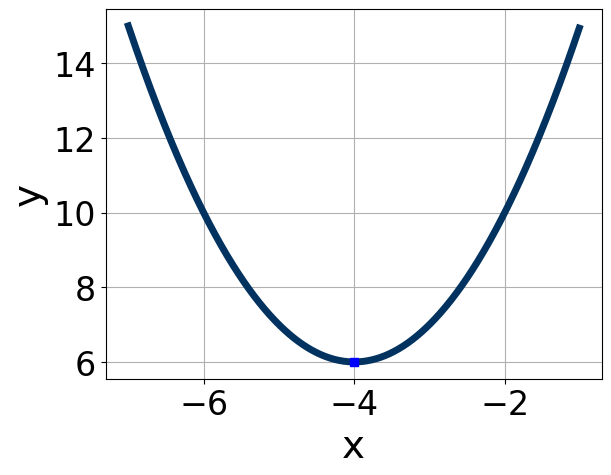
\includegraphics[width=0.5\textwidth]{../Figures/quadraticGraphToEquationC.png}
\end{center}
\begin{enumerate}[label=\Alph*.]
\item \( a \in [0.4, 1.8], \hspace*{5mm} b \in [-9, -3], \text{ and } \hspace*{5mm} c \in [21, 24] \)
\item \( a \in [-1.2, -0.2], \hspace*{5mm} b \in [-9, -3], \text{ and } \hspace*{5mm} c \in [-12, -8] \)
\item \( a \in [0.4, 1.8], \hspace*{5mm} b \in [6, 9], \text{ and } \hspace*{5mm} c \in [21, 24] \)
\item \( a \in [0.4, 1.8], \hspace*{5mm} b \in [6, 9], \text{ and } \hspace*{5mm} c \in [10, 11] \)
\item \( a \in [-1.2, -0.2], \hspace*{5mm} b \in [6, 9], \text{ and } \hspace*{5mm} c \in [-12, -8] \)

\end{enumerate} }
\litem{
Graph the equation below.\[ f(x) = (x+2)^2 + 16 \]\begin{enumerate}[label=\Alph*.]
\begin{multicols}{2}\item 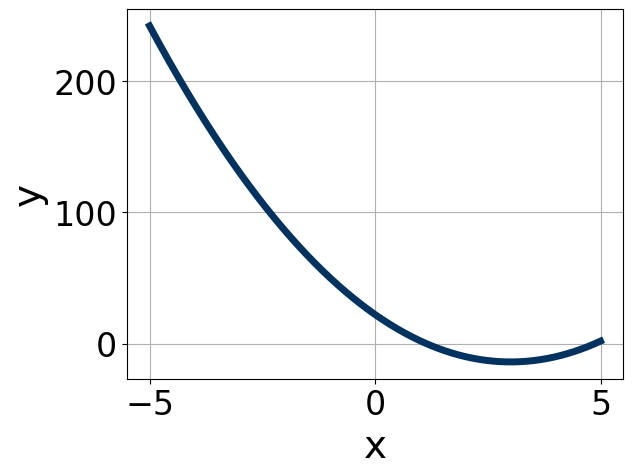
\includegraphics[width = 0.3\textwidth]{../Figures/quadraticEquationToGraphCopyAC.png}\item 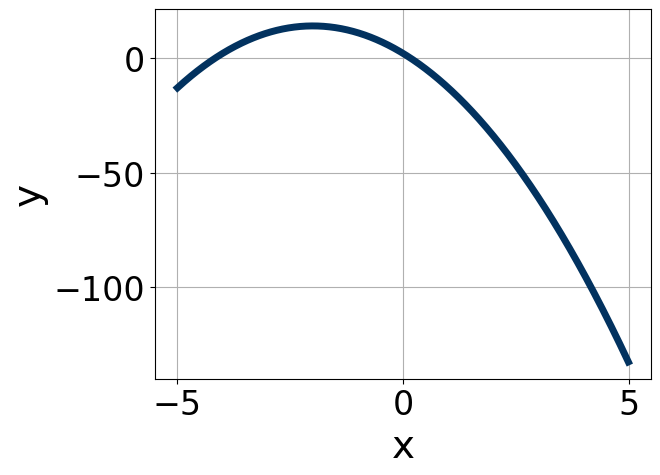
\includegraphics[width = 0.3\textwidth]{../Figures/quadraticEquationToGraphCopyBC.png}\item 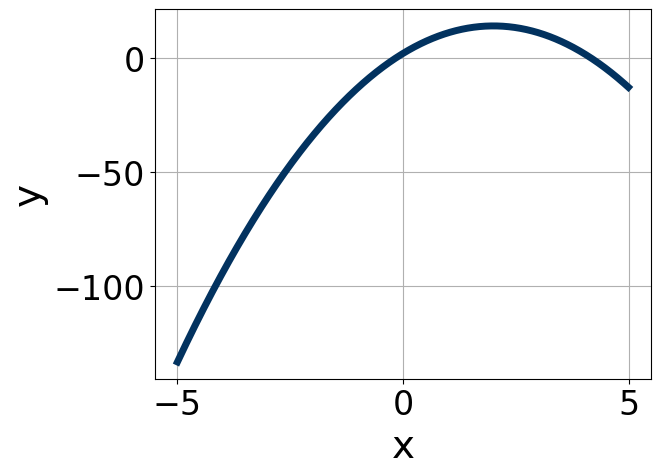
\includegraphics[width = 0.3\textwidth]{../Figures/quadraticEquationToGraphCopyCC.png}\item 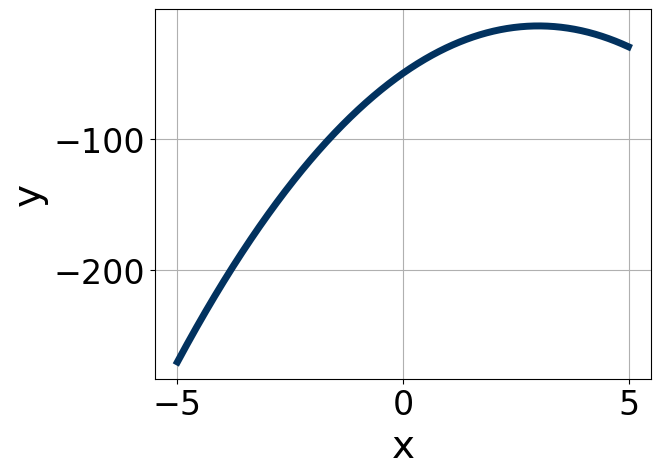
\includegraphics[width = 0.3\textwidth]{../Figures/quadraticEquationToGraphCopyDC.png}\end{multicols}\item None of the above.
\end{enumerate} }
\litem{
Write the equation of the graph presented below in the form $f(x)=ax^2+bx+c$, assuming  $a=1$ or $a=-1$. Then, choose the intervals that $a, b,$ and $c$ belong to.
\begin{center}
    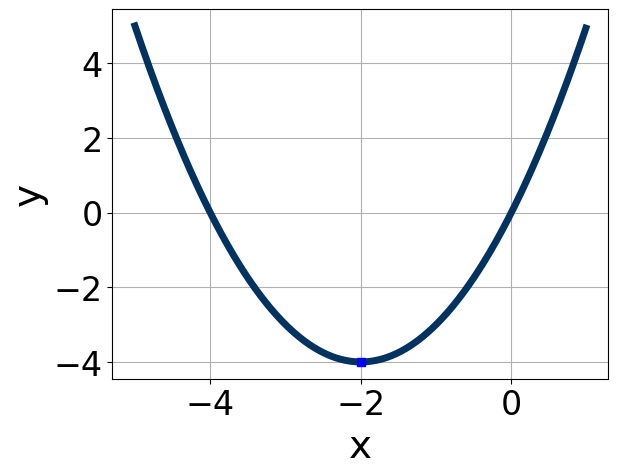
\includegraphics[width=0.5\textwidth]{../Figures/quadraticGraphToEquationCopyC.png}
\end{center}
\begin{enumerate}[label=\Alph*.]
\item \( a \in [-2, 0], \hspace*{5mm} b \in [1, 6], \text{ and } \hspace*{5mm} c \in [3, 6] \)
\item \( a \in [-2, 0], \hspace*{5mm} b \in [1, 6], \text{ and } \hspace*{5mm} c \in [-13, -8] \)
\item \( a \in [-2, 0], \hspace*{5mm} b \in [-7, 0], \text{ and } \hspace*{5mm} c \in [-13, -8] \)
\item \( a \in [1, 2], \hspace*{5mm} b \in [-7, 0], \text{ and } \hspace*{5mm} c \in [-7, 0] \)
\item \( a \in [1, 2], \hspace*{5mm} b \in [1, 6], \text{ and } \hspace*{5mm} c \in [-7, 0] \)

\end{enumerate} }
\litem{
Solve the quadratic equation below. Then, choose the intervals that the solutions belong to, with $x_1 \leq x_2$ (if they exist).\[ -20x^{2} +9 x + 2 = 0 \]\begin{enumerate}[label=\Alph*.]
\item \( x_1 \in [-0.2, 0.15] \text{ and } x_2 \in [0.33, 0.74] \)
\item \( x_1 \in [-0.83, -0.51] \text{ and } x_2 \in [-0.03, 0.33] \)
\item \( x_1 \in [-12.73, -11.88] \text{ and } x_2 \in [2.83, 3.48] \)
\item \( x_1 \in [-15.78, -14.86] \text{ and } x_2 \in [15.31, 15.79] \)
\item \( \text{There are no Real solutions.} \)

\end{enumerate} }
\litem{
Factor the quadratic below. Then, choose the intervals that contain the constants in the form $(ax+b)(cx+d); b \leq d.$\[ 24x^{2} +50 x + 25 \]\begin{enumerate}[label=\Alph*.]
\item \( a \in [4.69, 6.85], \hspace*{5mm} b \in [2, 10], \hspace*{5mm} c \in [3.3, 8.5], \text{ and } \hspace*{5mm} d \in [1, 10] \)
\item \( a \in [-0.88, 1.76], \hspace*{5mm} b \in [18, 22], \hspace*{5mm} c \in [-0.7, 1.7], \text{ and } \hspace*{5mm} d \in [26, 34] \)
\item \( a \in [1.77, 2.45], \hspace*{5mm} b \in [2, 10], \hspace*{5mm} c \in [10.9, 12.3], \text{ and } \hspace*{5mm} d \in [1, 10] \)
\item \( a \in [11.12, 12.58], \hspace*{5mm} b \in [2, 10], \hspace*{5mm} c \in [1.9, 2.9], \text{ and } \hspace*{5mm} d \in [1, 10] \)
\item \( \text{None of the above.} \)

\end{enumerate} }
\litem{
Solve the quadratic equation below. Then, choose the intervals that the solutions $x_1$ and $x_2$ belong to, with $x_1 \leq x_2$.\[ 25x^{2} -60 x + 36 = 0 \]\begin{enumerate}[label=\Alph*.]
\item \( x_1 \in [0.3, 0.52] \text{ and } x_2 \in [3.39, 4.17] \)
\item \( x_1 \in [29.74, 30.12] \text{ and } x_2 \in [28.62, 30.15] \)
\item \( x_1 \in [0.13, 0.39] \text{ and } x_2 \in [5.64, 6.62] \)
\item \( x_1 \in [1.05, 1.38] \text{ and } x_2 \in [0.13, 2.18] \)
\item \( x_1 \in [0.49, 0.71] \text{ and } x_2 \in [1.51, 2.9] \)

\end{enumerate} }
\litem{
Factor the quadratic below. Then, choose the intervals that contain the constants in the form $(ax+b)(cx+d); b \leq d.$\[ 54x^{2} +15 x -25 \]\begin{enumerate}[label=\Alph*.]
\item \( a \in [2.6, 5.7], \hspace*{5mm} b \in [-5, -4], \hspace*{5mm} c \in [17.86, 18.4], \text{ and } \hspace*{5mm} d \in [2, 6] \)
\item \( a \in [-1.5, 1.6], \hspace*{5mm} b \in [-31, -25], \hspace*{5mm} c \in [0, 1.33], \text{ and } \hspace*{5mm} d \in [45, 48] \)
\item \( a \in [6.3, 10.6], \hspace*{5mm} b \in [-5, -4], \hspace*{5mm} c \in [4.79, 6.55], \text{ and } \hspace*{5mm} d \in [2, 6] \)
\item \( a \in [17.6, 20.1], \hspace*{5mm} b \in [-5, -4], \hspace*{5mm} c \in [1.26, 4.1], \text{ and } \hspace*{5mm} d \in [2, 6] \)
\item \( \text{None of the above.} \)

\end{enumerate} }
\litem{
Graph the equation below.\[ f(x) = (x-4)^2 + 17 \]\begin{enumerate}[label=\Alph*.]
\begin{multicols}{2}\item 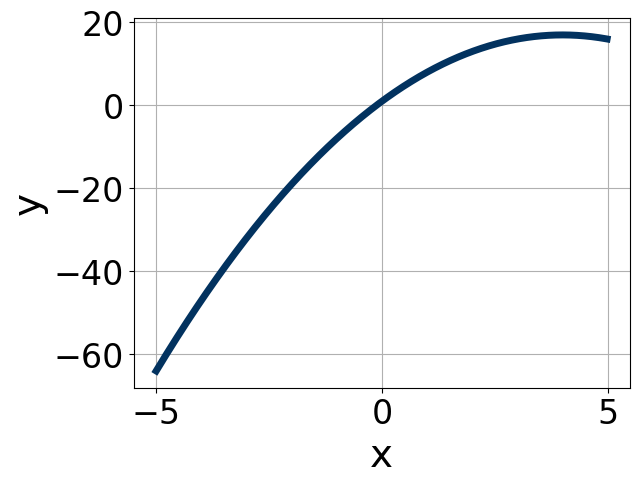
\includegraphics[width = 0.3\textwidth]{../Figures/quadraticEquationToGraphAC.png}\item 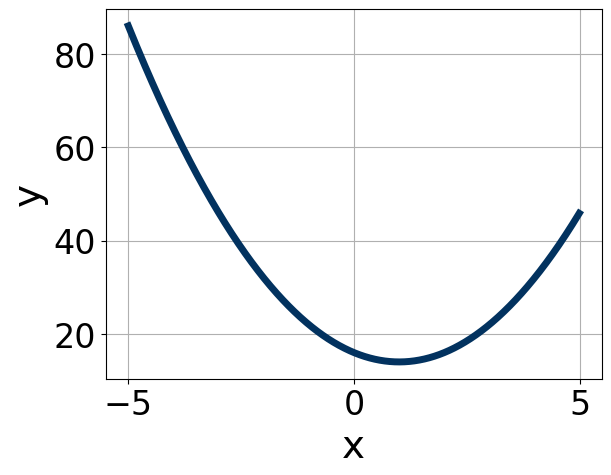
\includegraphics[width = 0.3\textwidth]{../Figures/quadraticEquationToGraphBC.png}\item 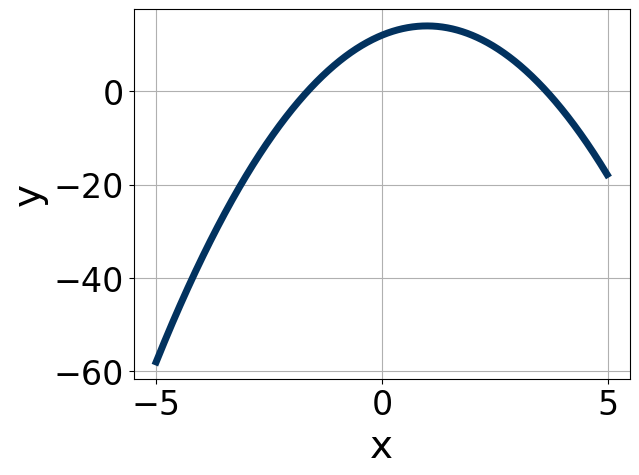
\includegraphics[width = 0.3\textwidth]{../Figures/quadraticEquationToGraphCC.png}\item 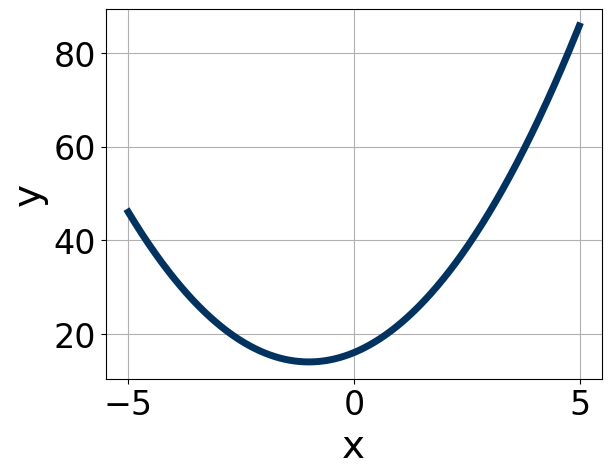
\includegraphics[width = 0.3\textwidth]{../Figures/quadraticEquationToGraphDC.png}\end{multicols}\item None of the above.
\end{enumerate} }
\end{enumerate}

\end{document}